\documentclass[PICOReport.tex]{subfiles}

\begin{document}

\begin{figure*}
%\vskip-3cm
\begin{center}
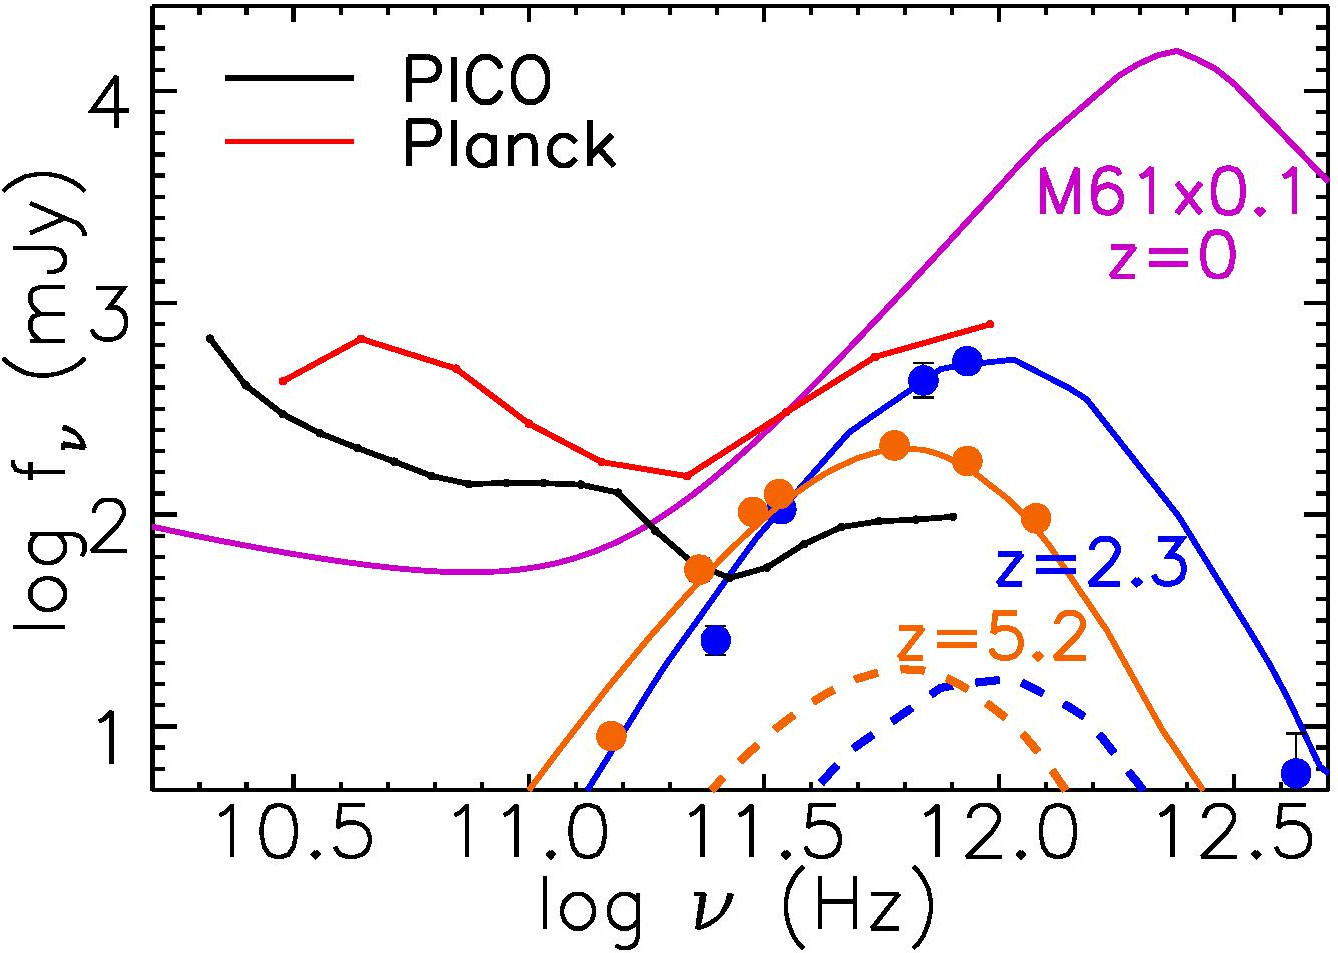
\includegraphics[width=0.41\columnwidth, trim={0 0 0 0cm}, clip]{images/fig_SED_PICO.jpg}
\hspace{0.75cm}
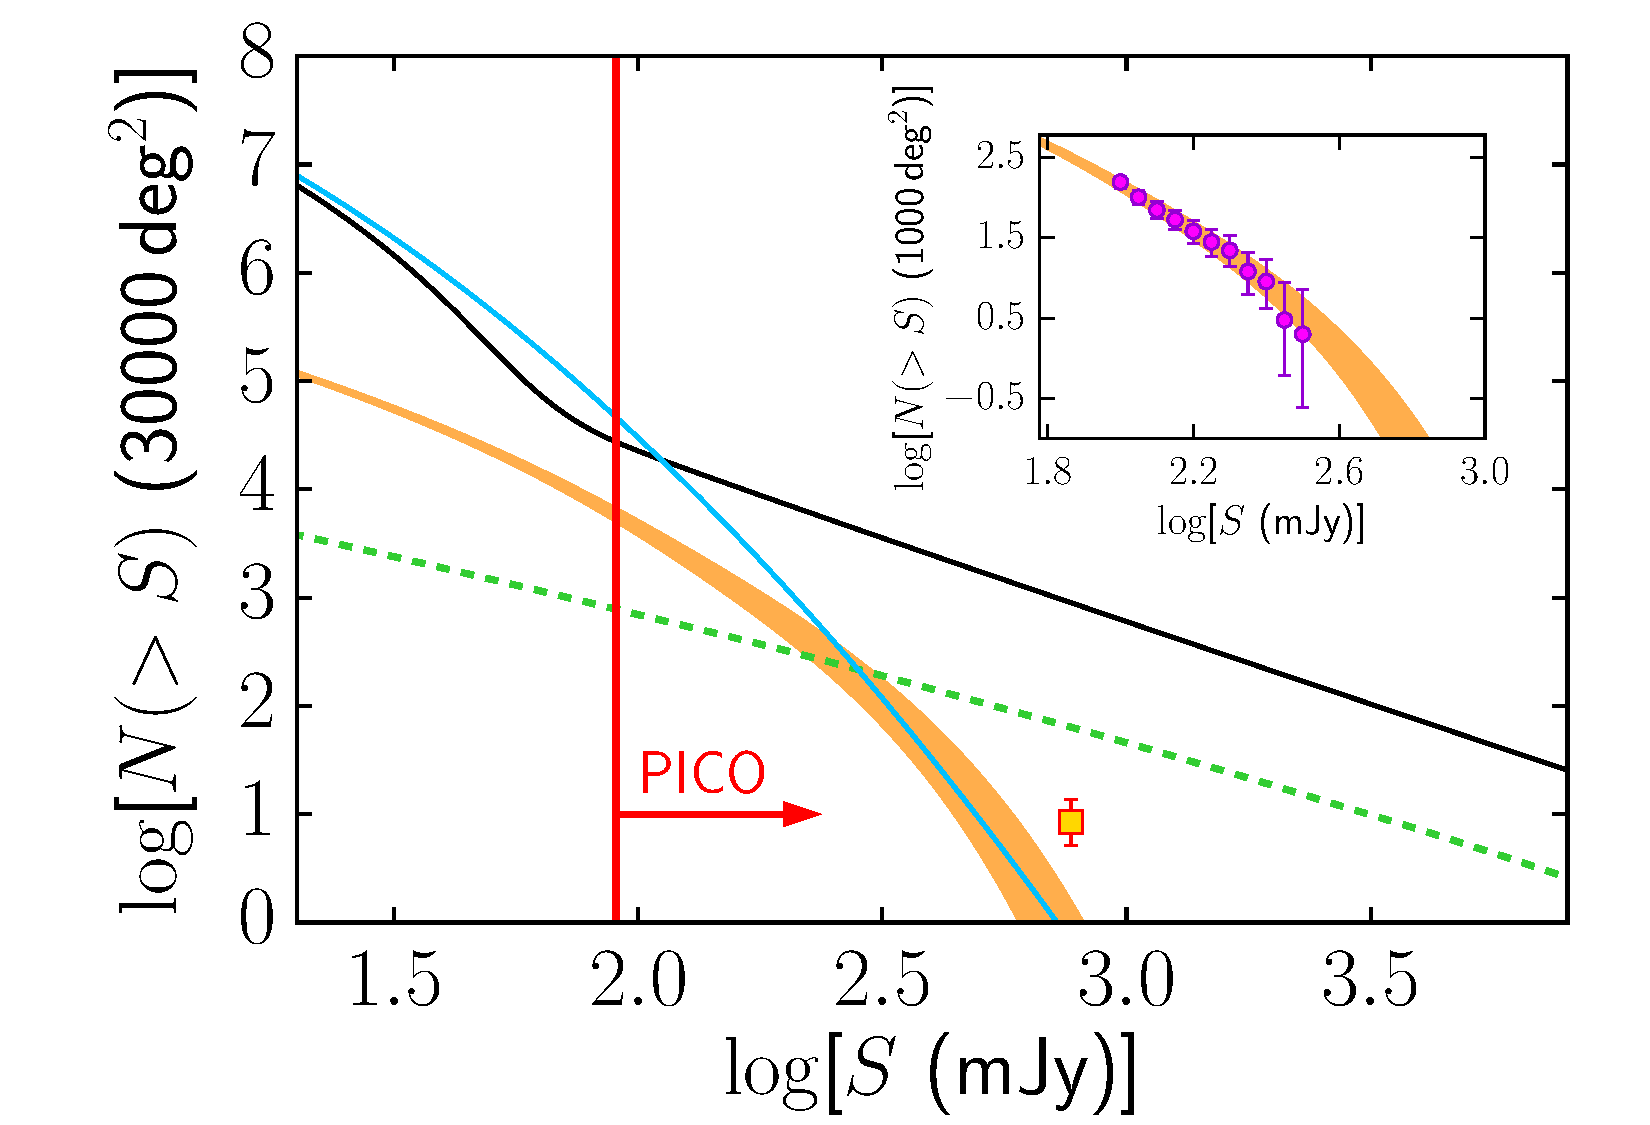
\includegraphics[width=0.4\columnwidth, trim={0 0 0 0cm}, clip]{images/NgtF_pico_NEW.pdf}
\vskip-0.3cm
\caption{\textbf{Left panel.} Example spectral energy distributions (SEDs) of dusty star-forming galaxies detectable by PICO, compared with its point source detection limits (black line) and with the \planck\ 90\% completeness limits (red line~\cite{PCCS2}). PICO will detect nearby galaxies, like M\,61 (magenta), whose SED was scaled down by a factor of ten, and high-$z$ strongly lensed galaxies, like SMM\,J2133-0102 (blue)  at $z=2.3$ \cite{Swinbank2010} and HLSJ$091828.6{+}514223$ (orange) at $z=5.2$ \cite{Combes2012}. The dashed lines are corrected for lensing magnification.  \textbf{Right panel.} Integral counts at $500\,\mu$m (600\,GHz) of unlensed, low-$z$ (black) and strongly lensed, high-$z$ (orange) star-forming galaxies based on fits of \textit{Herschel} counts (inset~\citep{Negrello2017lensed}), also shown are predicted radio source counts (green). The PICO detection region (right of vertical red line) will yield a factor of 1000 increase in strongly lensed galaxies relative to Planck (yellow square),
%the counts of unlensed galaxies have an Euclidean slope, indicative of low $z$.
and $\sim50,000$ proto-clusters (blue)~\citep{Negrello2017protocl}.}
\label{fig:SED3}
\end{center}
\vspace{-0.15in}
\end{figure*}

\subsubsection{Early phases of galaxy evolution}

PICO will have a crucial role in providing answers to major, still open issues on galaxy formation and evolution. Which are the main physical mechanisms shaping the galaxy properties~\citep{SilkMamon2012, SomervilleDave2015}: in situ processes, interactions, mergers, or cold flows  from the intergalactic medium? How do feedback processes work? To settle these issues we need direct information on the structure and the dynamics of high-$z$ galaxies. But these are compact, with typical sizes of 1--2~kpc~\cite{Fujimoto2018}), corresponding to angular sizes of 0.1--0.2~arcsec at $z\simeq 2$--3. Thus they are hardly resolved even by ALMA and by HST. If they are resolved, high enough \ac{SNR} per resolution element are achieved only for the brightest galaxies, which are probably not representative of the general population.

Strong gravitational lensing provides a solution to these problems. PICO will detect galaxies whose flux densities are boosted by large factors; see the right panel of Fig.~\ref{fig:SED3}. Since lensing conserves the surface brightness, the effective angular size is stretched on average by a factor $\mu^{1/2}$, where $\mu$ is the gravitational magnification, thus substantially increasing the resolving power. A spectacular example are ALMA observations of the strongly lensed galaxy PLCK\_G244.8\-+54.9 at $z \simeq 3.0$  with $\mu \simeq 30$~\citep{Canameras2017ALMA}. ALMA observation with a $0.1''$ resolution reached the astounding spatial resolution of $\simeq 60\,$pc, substantially smaller than the size of Galactic giant molecular clouds. Other high-$z$ galaxies spatially resolved thanks to gravitational lensing, with less extreme magnifications, are reported by~\citet{Dye2018}, and others~\citep{Lamarche2018, Sharda2018}.

Ca\~{n}ameras et al.~\citep{Canameras2017ALMA} have also obtained CO spectroscopy, measuring the kinematics of the molecular gas with an uncertainty of 40--50~km/s. This spectral resolution makes possible a direct investigation of massive outflows driven by AGN feedback at high $z$. In this way \citet{Spilker2018} were able to detect a fast (800 km/s) molecular outflow due to feedback in a strongly lensed galaxy at $z=5.3$. The outflow carries mass at a rate close to the SFR and can thus remove a large fraction of the gas available for star-formation.

\textit{Herschel} surveys have demonstrated that, at the PICO detection limit at $\simeq 500\,\mu$m (600\,GHz), about 25\% of all detected extragalactic sources are strongly lensed; for comparison, at optical/near-IR and radio wavelengths, were intensive searches have been carried out for many years, the yield is of only 0.1\%, i.e. more than two orders of magnitude lower \cite{Treu2010}. To add to the extraordinary sub-mm bonanza, the selection of strongly lensed galaxies detected by sub-mm surveys is extremely easy because of their peculiar sub-mm colors -- see the left panel of Fig.~\ref{fig:SED3} -- resulting in a selection efficiency close to 100\% \citep{Negrello2010}.

A straightforward extrapolation of the \textit{Herschel} counts to the much larger area covered by PICO shows that its surveys will yield $\sim 4,500$ strongly lensed galaxies with a redshift distribution peaking at $2\simlt z \simlt 3$ \cite{Negrello2017lensed} but extending up to $z> 5$; see the left panel of Fig.~\ref{fig:SED3}. If objects like the $z=5.2$ strongly lensed galaxy HLSJ$091828.6+514223$ exist at higher redshifts, they will be detectable by PICO up to $z>10$.

An intensive high spectral and spatial resolution follow up campaign of such a large sample will be challenging but also extremely rewarding since it will allow a giant leap forward towards the understanding of the processes driving early galaxy evolution, in addition to opening many other exciting prospects both on the astrophysical and on the cosmological side (cf., e.g., ref. \cite{Treu2010}). The PICO all-sky surveys will select the brightest objects in the sky, maximizing the efficiency of the effort.

\subsubsection{Early phases of cluster evolution}

PICO will open a new window for the investigation of early phases of cluster evolution, when their member galaxies were actively star forming but the hot IGM was not necessarily in place. In this phase, traditional approaches to cluster detection (X-ray and SZ surveys, searches for galaxy red sequences) work only for the more evolved objects; indeed these methods have yielded only a handful of confirmed proto-clusters at $z\simgt 1.5$ \cite{Overzier2016}\footnote{More high-$z$ proto-clusters have been found targeting the environment of tracers of very massive halos, such as radio-galaxies, QSOs, sub-mm galaxies. These searches are however obviously biased.}.
\textit{Planck} has demonstrated the power of low-resolution surveys for the study of large-scale structure  \cite{Planck2016high_z} but its resolution was too poor to detect individual proto-clusters \cite{Negrello2017protocl}.  Studies of the high-$z$ 2-point correlation function \cite{Chen2016, Negrello2017protocl} and \textit{Herschel} images of the few sub-mm bright protoclusters detected so far, at $z$ of up to 4 \cite{Ivison2013, Wang2016, Oteo2018}, all of which will be detected by PICO, indicate sizes of $\simeq 1'$ for the cluster cores, nicely matching the PICO FWHM at the highest frequencies.

PICO will detect many tens of thousands of these objects -- this is the blue line in the right-hand panel of Fig.~\ref{fig:SED3} -- as peaks in its sub-mm maps, in addition to the evolved ones, detected by the SZ effect. This will constitute a real breakthrough in the observational validation of the formation history of the most massive dark matter halos, traced by clusters, a crucial test of models for structure formation. Follow-up observations will characterize the properties of member galaxies, probing the galaxy evolution in dense environments and shedding light on the complex physical processes driving it.

\subsubsection{Additional products of PICO surveys}

PICO will also yield a complete census of cold dust, available to sustain star formation in the nearby Universe, by detecting tens of thousands galaxies mostly at $z\simlt 0.1$. Its statistics will allow us to investigate the distribution of such dust as a function of galaxy properties (morphology, stellar mass, etc.).

Moreover, PICO will increase by orders of magnitude the number of blazars selected at sub-mm wavelengths and will determine the SEDs of many hundreds of them up to 800\,GHz and up to $z> 5$. Blazar searches are the most effective way to sample the most massive BHs at high $z$ because of the Doppler boosting of their flux densities. Its surveys of the largely unexplored mm/sub-mm spectral region will also offer the possibility to discover new transient sources \cite{Metzger2015} or events, such as blazar outbursts.

PICO will also make a giant leap forward in the determination of
polarization properties of both radio sources and of dusty galaxies over a frequency range where ground based surveys are impractical or impossible. Thanks to its high sensitivity, it will detect in polarization both populations over a substantial flux density range, determining directly, for the first time, number counts in polarized flux density and allowing an accurate correction for their contamination of CMB maps.

The anisotropy of the \ac{CIB}, produced by dusty star-forming galaxies in a wide redshift range, is an excellent probe of both the history of star formation and the link between
galaxies and dark matter across cosmic time. The \planck\ collaboration derived values of the star formation rate up to redshifts z$\mathrm{\sim 4}$~\cite{2014A&A...571A..30P,2014A&A...571A..18P,madau2014}).
It was quantified in \cite{Wu:2016hej} that the increased \ac{SNR} and frequency coverage enabled by PICO will enable an order of magnitude improvement on the statistical errors on these parameters.
Similar improvement will be achieved in constraining $M_{\mathrm{eff}}$, the galaxy halo mass that is most efficient in producing star formation activity. PICO extra-frequencies and increased sensitivity to Galactic dust polarization will provide enhanced means to separate the largely unpolarized \ac{CIB} from polarized Galactic dust, the limiting factor towards more extended reliable legacy \ac{CIB} maps.

%For example, a key parameter in
%simulations of the angular power spectrum of the \ac{CIB}
%is $M_{\mathrm{eff}}$, the galaxy halo mass that is most efficient in producing star
%formation activity. Comparing measurements of the power spectrum to simulations
%constrains this parameter, which informs structure formation models. Current models and measurements
%find $M_{\mathrm{eff}}\sim 10^{12}$ solar masses with about $\mathrm{10\%}$ uncertainty.
%The CMB Probe will constrain this parameter at the percent level.

%Dusty star-forming galaxies trace the underlying dark matter
%field in a broad redshift range. Therefore, a wealth of information will be extracted by
%correlating the anisotropy in the \ac{CIB}
%with multiple dark matter tracers including catalogs of galaxies and quasars,
%and maps of the $\gamma$-ray and the X-ray background~\cite{serra2014,wang2015,cooray2016}.
%These cross-correlations will provide an additional probe of the star formation history, and they will shed light on the interaction between
%light and matter in a broad wavelength range. \comred{the paragraph starts with dark matter, but ends
%with SFR ..?}


\end{document}

%%%%%%%%%%%%%%%%%%%%%%%%%%%%%%%
